\begin{figure}[t]
    \centering
    \begin{subfigure}{0.45\textwidth}
    	\centering
    	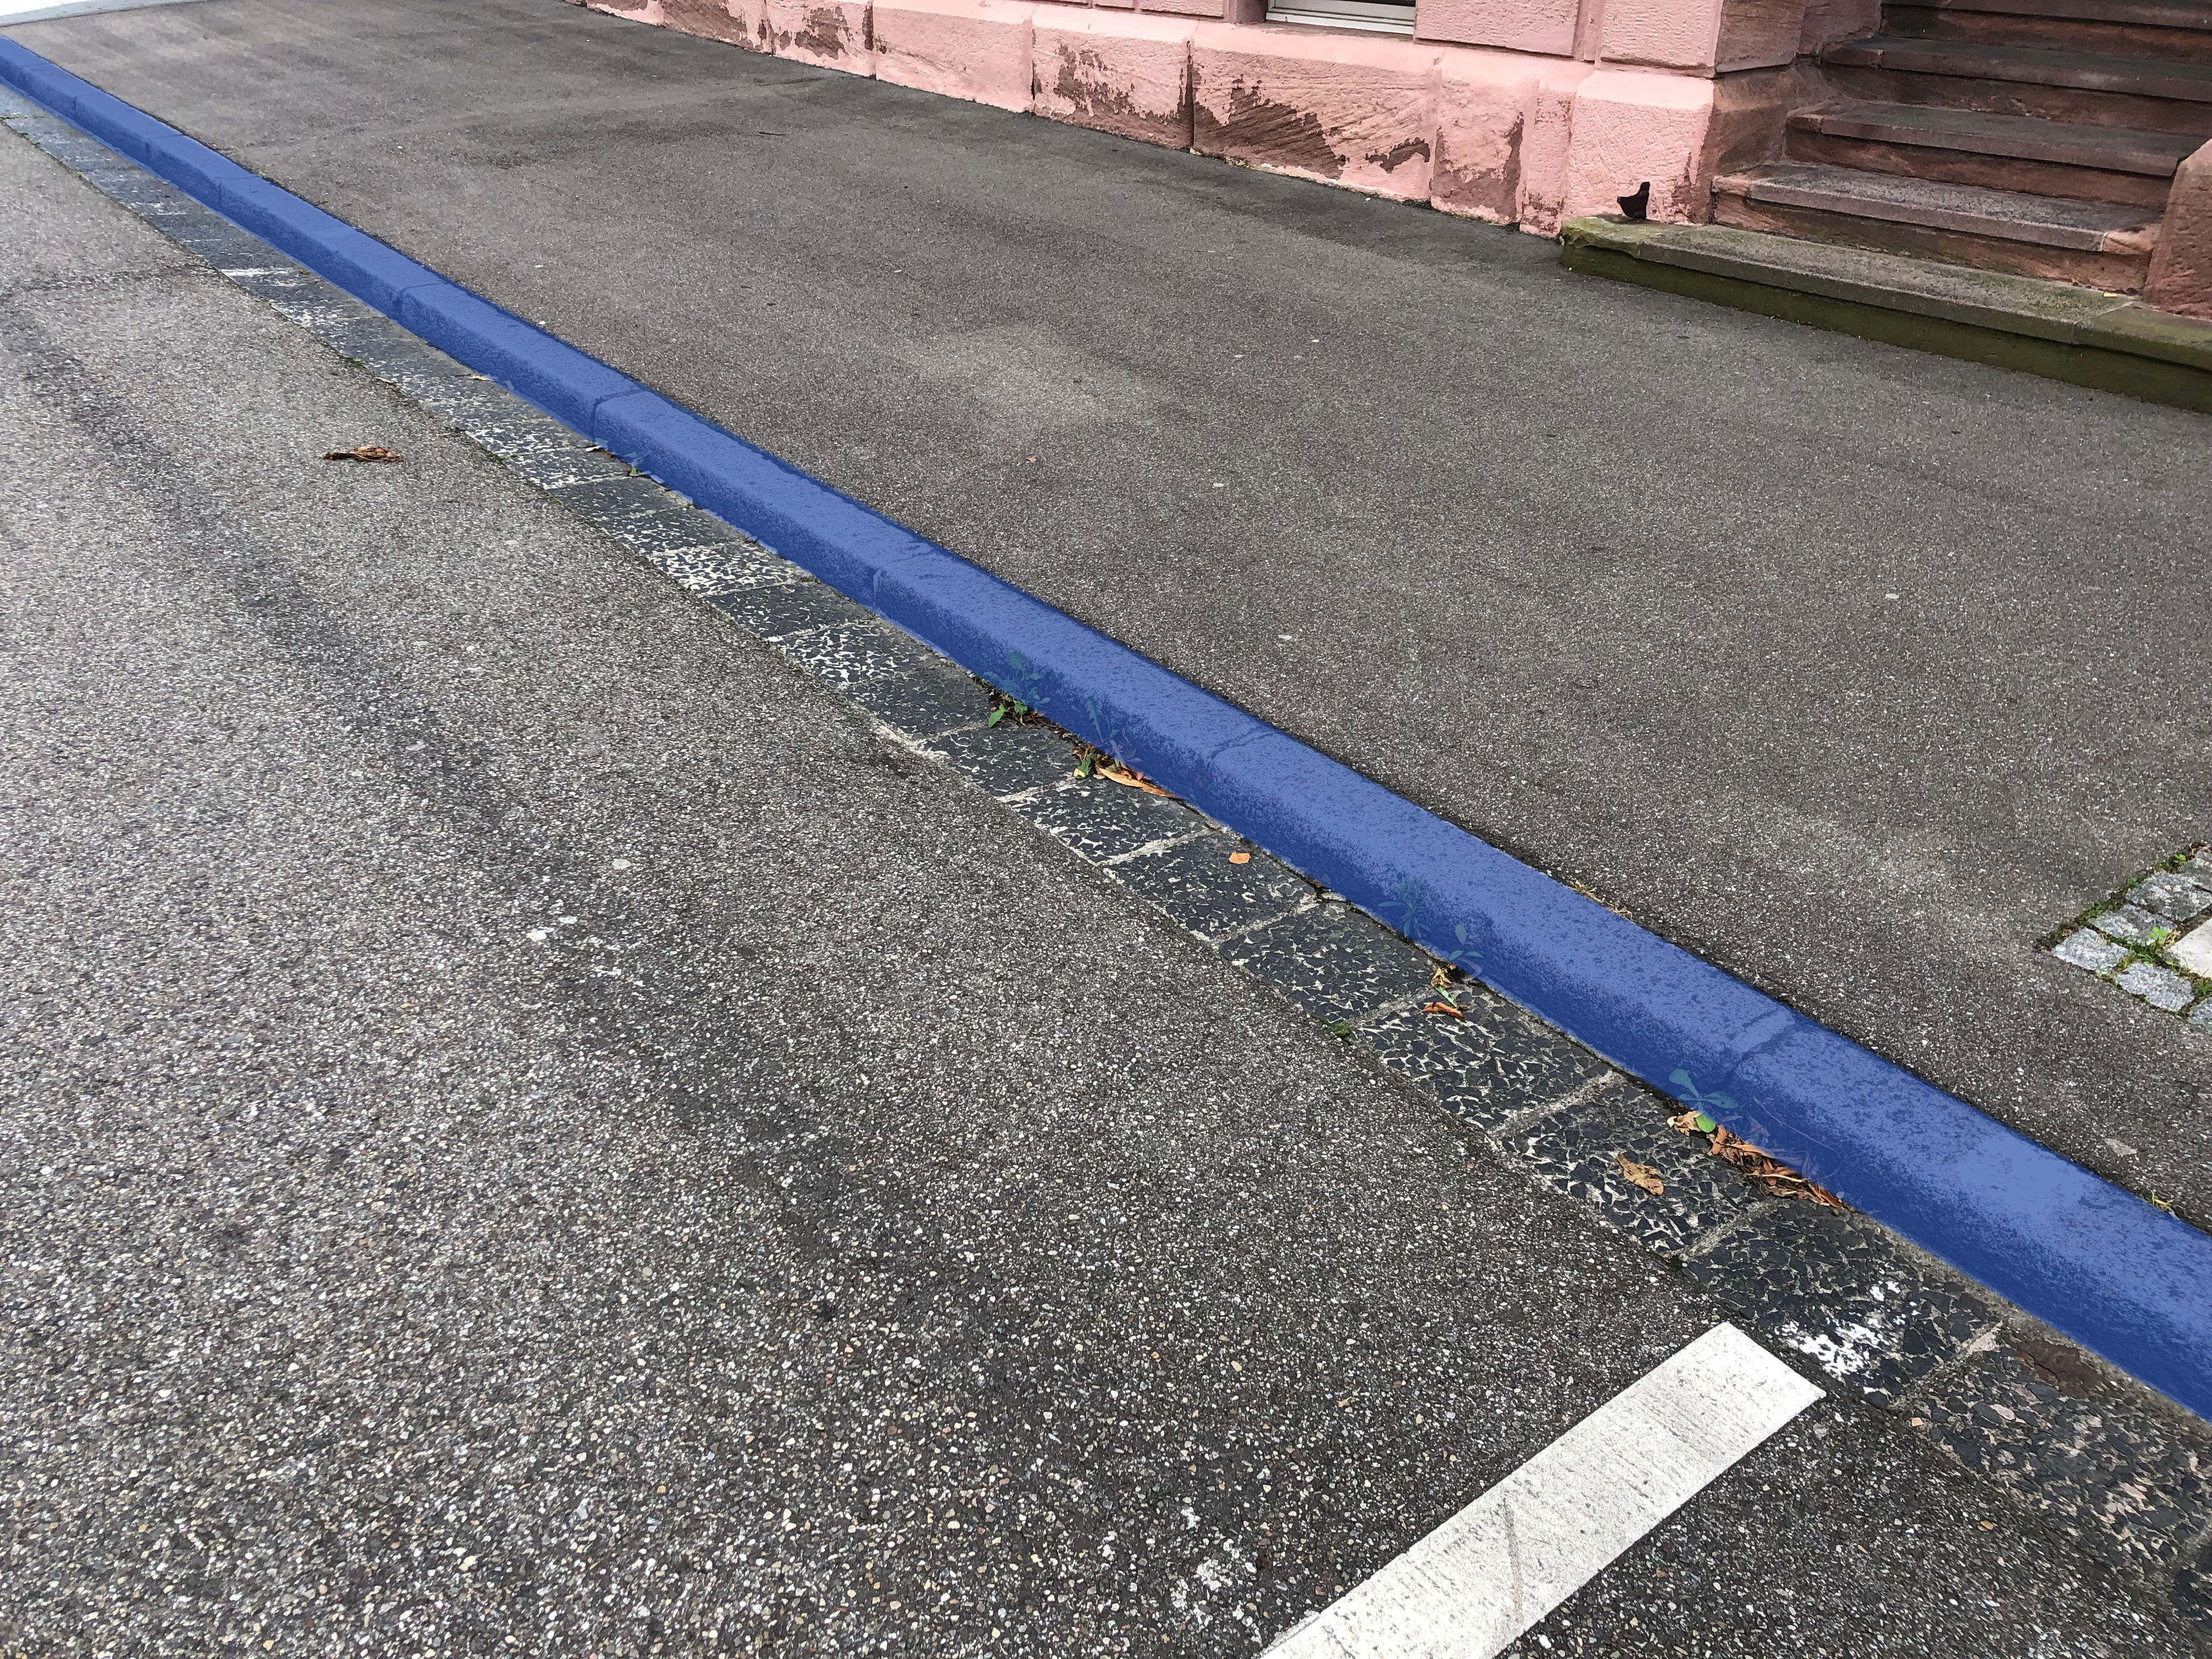
\includegraphics[width=0.9\textwidth]{figures/background/curb.jpeg} % first figure
    	\caption{An example of a sidewalk with a curb, the curb highlighted in blue.} \label{fig:background-curb}
    \end{subfigure}
	\hfill
    \begin{subfigure}{0.45\textwidth}
        \centering
        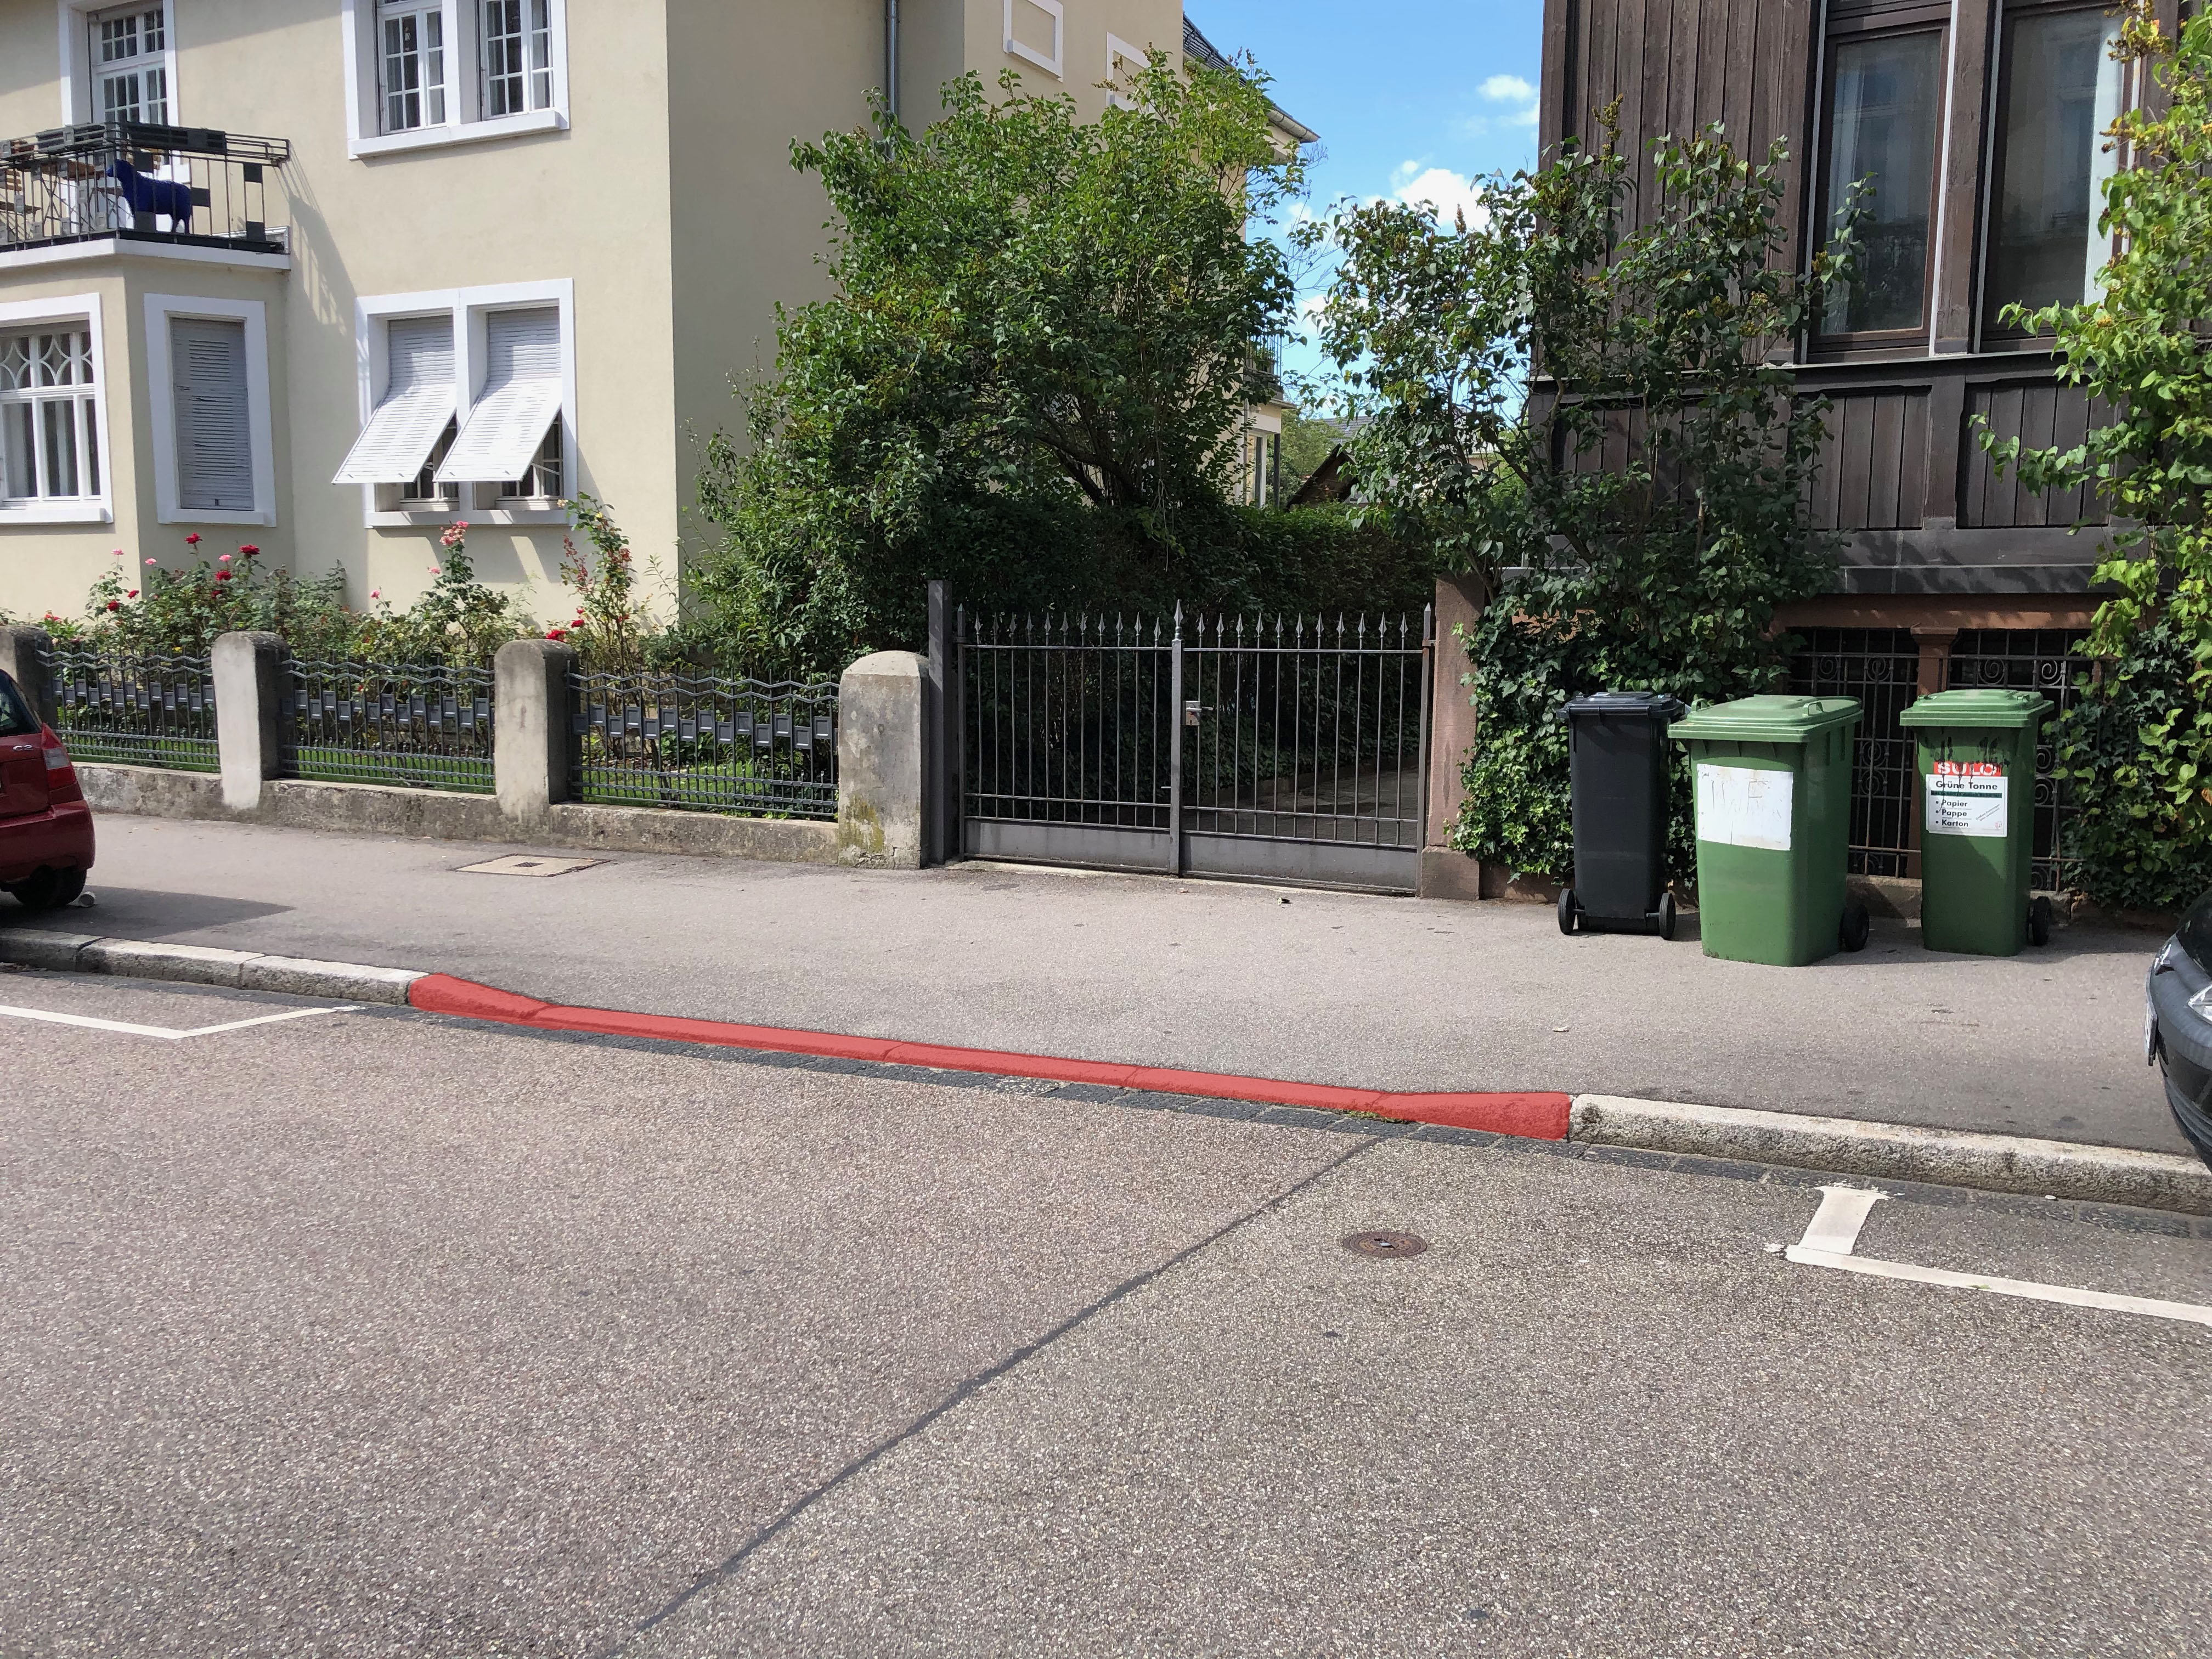
\includegraphics[width=0.9\textwidth]{figures/background/curbcut.jpeg} % second figure
        \caption{An example of a sidewalk with a curb cut, the curb cut highlighted in red.} \label{fig:background-curbcut}
    \end{subfigure}
	\caption[Curbs and curb cuts]{An example of a curb and a curb cut. Being able to segment these structures is one of the goals of this thesis.}
\end{figure}